%! TEX root = main.tex

\graphicspath{{00_Images/08_chapter/}}

\chapter{Flat Power, Efficiency, and Thiele-Small Parameters}
\label{ch:efficiency}

The previous chapter showed that above resonance the diaphragm acceleration is constant, independent of frequency.
This chapter traces the consequence of that result for the radiated acoustic power, derives the efficiency of the electrodynamic loudspeaker as a complete transducer, and introduces the compact set of parameters needed to characterize any driver independently of the specific equivalent circuit used during analysis.

\section{Frequency-Independent Acoustic Power}
\label{sc:81}

The mean acoustic power radiated by the loudspeaker in the band above resonance is:
\[
\overline{W_A} = R_{MR} u_{C,\mathrm{RMS}}^2
\]
where \(R_{MR} = S_D^2 R_{AR}\) is the mechanical radiation resistance and \(u_C\) is the diaphragm velocity.
At first glance, since \(u_C \propto 1/f\) in the mass-controlled regime, one might expect \(\overline{W_A} \propto 1/f^2\), implying a steadily decreasing radiated power.
However, the radiation resistance is not constant: as shown in chapter \ref{ch:sound_radiation}, for a piston with \(ka \ll 1\) the specific radiation resistance rises as:
\[
R_s \approx \frac{a^2 \rho_0}{2c} \omega^2 \propto \omega^2
\]
Referring this to the mechanical domain, \(R_{MR} = S_D R_s \propto \omega^2\).
The two frequency dependences cancel exactly:
\[
\overline{W_A} = R_{MR} u_{C,\mathrm{RMS}}^2 \propto \omega^2 \cdot \frac{1}{\omega^2} = \text{const}
\]
Substituting the explicit expressions for \(u_C\) in the mass-controlled regime and for \(R_{MR}\) in the low-frequency limit:
\begin{equation}
    \overline{W_A} = \frac{v_{g,\mathrm{RMS}}^2 (Bl)^2 S_D^2 \rho_0}{(R_g + R_{EC})^2 \pi c M_{MS}^2}
    \label{eq:flatPower}
\end{equation}
This result is remarkable: the radiated acoustic power is independent of frequency for all \(f\) in the range \(f_s < f < f_0\), where \(f_0 = c/(2\pi a)\) is the piston cutoff frequency.
The physical picture is that, while the diaphragm moves with diminishing velocity as frequency rises, it simultaneously becomes a better radiator because its size grows relative to the shrinking wavelength.
The two effects balance with arithmetic precision, maintaining a constant acoustic output.
The design implication is direct: to obtain a flat acoustic power response over a given bandwidth, the working range of the driver must lie within the interval \(f_s < f < f_0\), making the choice of \(f_s\) and diaphragm radius \(a\) the two primary design variables.

\section{Loudspeaker Efficiency}
\label{sc:82}

The electroacoustic efficiency \(\varepsilon\) of the loudspeaker is defined as the ratio of the mean radiated acoustic power to the mean electrical power absorbed from the source:
\[
\varepsilon = \frac{\overline{W_A}}{\overline{W_E}}
\]
The mean electrical power delivered to the loudspeaker terminals is approximately \(\overline{W_E} \approx v_{g,\mathrm{RMS}}^2/R_{EC}\), assuming the source resistance is negligible compared to the voice-coil resistance (\(R_g \ll R_{EC}\)).
Dividing equation \eqref{eq:flatPower} by this expression:
\begin{equation}
    \varepsilon = \frac{(Bl)^2 \rho_0}{\pi c R_{EC}}\left(\frac{S_D}{M_{MS}}\right)^2
    \label{eq:efficiency}
\end{equation}
Equation \eqref{eq:efficiency} reveals the three principal levers available to the designer for improving efficiency: increasing the force factor \(Bl\) (stronger magnet, more wire in the gap), reducing the voice-coil resistance \(R_{EC}\), and maximizing the ratio \(S_D/M_{MS}\) (large, lightweight diaphragm).

\paragraph{Numerical example} Inserting typical values for a commercial woofer:
\[
Bl = \SI{10}{\newton\per\ampere}, \quad
R_{EC} = \SI{6}{\ohm}, \quad
S_D = \pi (0.1)^2 \approx \SI{0.03}{\meter\squared}
\]
\[
M_{MS} = M_{MD} + 2M_{M1} = 0.1 + 0.006 \approx \SI{0.2}{\kilo\gram}, \quad
\rho_0 = \SI{1.2}{\kilo\gram\per\cubic\meter}, \quad
c = \SI{343}{\meter\per\second}
\]
the efficiency evaluates to:
\[
\varepsilon \approx 0.15\%
\]
Less than two thousandths of the electrical energy supplied by the amplifier is converted into radiated sound; the remainder is dissipated as heat in the voice coil, the suspension, and the magnetic circuit.
This extraordinarily low efficiency is not a design failure but a fundamental consequence of the large impedance mismatch between the stiff, heavy mechanical system and the compliant, light acoustic medium.
Despite this, the electrodynamic loudspeaker remains the dominant transducer technology because its efficiency, though low in absolute terms, is achievable at high power levels with good linearity and in a compact, reproducible form.

\begin{figure}[!htb]
    \centering
    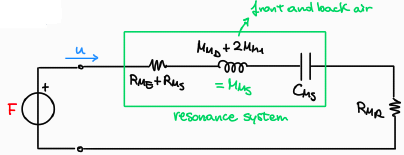
\includegraphics[width=0.60\linewidth]{loudspeaker_elec_scheme.png}
    \caption{Complete equivalent circuit of the loudspeaker at low-to-mid frequencies, referred to the electrical domain. The efficiency \(\varepsilon \approx 0.15\%\) follows from the ratio of the radiation resistance element to the total electrical losses}
\end{figure}

\section{The Thiele-Small Parameters}
\label{sc:83}

Any two engineers who measure the same loudspeaker must obtain the same small-signal behavior, regardless of which equivalent circuit model or which analogy they prefer.
This requirement motivates a compact, model-independent set of measurable parameters that fully characterize the driver near resonance.
The Thiele-Small parameter set, developed by Neville Thiele and Richard Small in the early 1970s, has become the universal standard in loudspeaker datasheets.
Six fundamental parameters are sufficient to reconstruct all elements of the equivalent circuit and to predict the in-box frequency response:

\begin{itemize}
    \item \(R_{EC}\): the DC resistance of the voice coil, measured in \si{\ohm}.
    \item \(Q_{ES}\): the electrical quality factor, quantifying the electromagnetic damping at resonance.
    \item \(Q_{MS}\): the mechanical quality factor, quantifying the suspension damping at resonance.
    \item \(f_s\): the free-air fundamental resonance frequency, in \si{\hertz}, given by equation \eqref{eq:resonanceFrequency}.
    \item \(S_D\): the effective piston area of the diaphragm, in \si{\meter\squared}, typically approximated as the area enclosed by the midpoint of the surround.
    \item \(V_{AS}\): the equivalent suspension volume, in \si{\meter\cubed} or liters, defined below.
\end{itemize}

From these six quantities, all derived parameters follow algebraically:
\[
C_{MS} = \frac{V_{AS}}{S_D^2 \rho_0 c^2}, \qquad
M_{MS} = \frac{1}{(2\pi f_s)^2 C_{MS}}, \qquad
R_{MS} = \frac{1}{Q_{MS}}\sqrt{\frac{M_{MS}}{C_{MS}}}
\]
\[
Bl = \sqrt{\frac{R_{EC}}{2\pi f_s Q_{ES} C_{MS}}}, \qquad
Q_{TS} = \frac{Q_{ES} Q_{MS}}{Q_{ES} + Q_{MS}}
\]

\section{Equivalent Suspension Volume}
\label{sc:84}

The equivalent suspension volume \(V_{AS}\) is the parameter that links the mechanical compliance of the suspension to a volume of air, making it directly comparable to enclosure volumes in box design.

\subsection{Physical Definition}
\label{ssc:841}

The acoustic compliance of a rigid sealed volume \(V_0\) of air undergoing adiabatic compression is:
\[
C_A = \frac{V_0}{\gamma P_0} \approx \frac{V_0}{\rho_0 c^2}
\]
where \(\gamma \approx 1.4\) is the ratio of specific heats and \(P_0\) is the ambient pressure.
The mechanical compliance \(C_{MS}\) of the suspension, when referred to the acoustic domain through the diaphragm area, defines an equivalent acoustic compliance:
\[
C_{AS} = {C_{MS}}{S_D^{2}}
\]
Setting this equal to \(C_A\) and solving for the volume:
\begin{equation}
    V_{AS} = C_{AS} \rho_0 c^2 = C_{MS} S_D^2 \rho_0 c^2
    \label{eq:VAS}
\end{equation}
The parameter \(V_{AS}\) is therefore the volume of air that, when sealed in a rigid container and compressed adiabatically, presents exactly the same acoustic compliance as the loudspeaker suspension.
Numerically, a woofer with a soft suspension and a large diaphragm can have \(V_{AS}\) of tens or even hundreds of liters; a tweeter with a stiff diaphragm typically has \(V_{AS}\) below one liter.

\subsection{The Syringe Analogy}
\label{ssc:842}

The concept of acoustic compliance as an air spring is most vividly demonstrated by a simple experiment: consider a medical syringe with its opening sealed by a thumb.
When the plunger is pushed inward, the trapped air is compressed and a restoring pressure builds up proportionally to the displacement, exactly as a mechanical spring restores a displaced mass.
Releasing the plunger, the compressed air pushes it back to its original position.
The analogy with a loudspeaker enclosure is direct: the volume of air sealed inside a closed-box cabinet plays the same role as the syringe volume.
The box air acts as an additional spring in series with the suspension, stiffening the total compliance and raising the resonance frequency above the free-air value \(f_s\).
The smaller the enclosure volume \(V_B\) relative to \(V_{AS}\), the stiffer the air spring and the greater the upward shift in resonance.
The ratio \(V_{AS}/V_B\) therefore quantifies how much the enclosure loads the suspension, and \(V_{AS}\) itself is the natural reference volume for enclosure design: a box of volume \(V_B = V_{AS}\) doubles the total stiffness, raising the resonance frequency by a factor of \(\sqrt{2}\).
More generally, the closed-box resonance frequency is:
\[
f_c = f_s \sqrt{1 + \frac{V_{AS}}{V_B}}
\]
This relation, together with equation \eqref{eq:Qts} and the known \(Q_{TS}\), allows the entire in-box frequency response to be predicted from the six Thiele-Small parameters before any physical enclosure is built.
The compactness and universality of the Thiele-Small framework account for its adoption as the standard specification language for the entire loudspeaker industry.
